
%(BEGIN_QUESTION)
% Copyright 2010, Tony R. Kuphaldt, released under the Creative Commons Attribution License (v 1.0)
% This means you may do almost anything with this work of mine, so long as you give me proper credit

Suppose someone who does not know what they're doing installs two control valves in the same gas line, controlled by two different PID controllers.  Each controller has P, I, and D actions active, and each one has its own local setpoint value set to 50\% of measurement range:

$$\includegraphics[width=15.5cm]{i04507x01.eps}$$

\vskip 10pt

Explain how these two controllers will react if the total gas flow rate into the receiver vessel from lines A and B exceeds the total gas flow out of the receiver vessel through lines C and D.  Specifically, identify whether each control valve will {\it open fully}, {\it close fully}, {\it throttle}, or {\it oscillate} after the system achieves its final state over time.

\vskip 100pt

Explain how these two controllers will react if the total gas flow rate into the receiver vessel from lines A and B is less than the total gas flow out of the receiver vessel through lines C and D by an amount greater than the setpoint of the flow controller.  Specifically, identify whether each control valve will {\it open fully}, {\it close fully}, {\it throttle}, or {\it oscillate} when the system achieves its final state over time.

\underbar{file i04507}
%(END_QUESTION)





%(BEGIN_ANSWER)

I suggest awarding 2.5 points for each correct controller response.

\vskip 10pt

Explain how these two controllers will react if the total gas flow rate into the receiver vessel from lines A and B exceeds the total gas flow out of the receiver vessel through lines C and D:

\begin{itemize}
\item{} FIC valve winds fully open
\item{} PIC valve winds fully closed
\end{itemize}

\vskip 10pt

Explain how these two controllers will react if the total gas flow rate into the receiver vessel from lines A and B is less than the total gas flow out of the receiver vessel through lines C and D by an amount greater than the setpoint of the flow controller: 

\begin{itemize}
\item{} FIC valve throttles
\item{} PIC valve winds fully open
\end{itemize}



%(END_ANSWER)





%(BEGIN_NOTES)

{\bf This question is intended for exams only and not worksheets!}.

%(END_NOTES)


